\subsection{Statistische Analyse von Höhendaten}
\usetikzlibrary{decorations.pathreplacing}
Ausserhalb der gewöhnlichen statistischen Analyse, die wir
hier als bekannt voraussetzen, führen wir hier weitere Werkzeuge
ein, die sich spezial für die Analyse rauer Oberflächen bzw. 
Gitterstrukturen als nützlich erweisen\cite{gwyddion}. Zunächst
gehen wir davon aus, dass uns die Mikroskopiedaten als 
$N \times M$ Vektorfeld vorliegen (N Zeilen und M Spalten der
Matrix der Bilddaten, ). Die tatsächliche Fläche der Daten
nennen wir nun $L_x \times L_y$, wobei 
wir ObdA nehmen nun annehmen, dass die Abstände
zwischen den Datenpunkten $\Delta$ betrage 
(siehe Abbildung~\ref{fig:stat1}). 

\begin{SCfigure}
\caption{Das Vektorfeld der Mikroskopiedaten besteht aus 
$N \times M$ Höhendaten aus $\mathbb{R}$, wobei die tatsächliche 
Fläche $L_x \times L_y$ beträgt.}

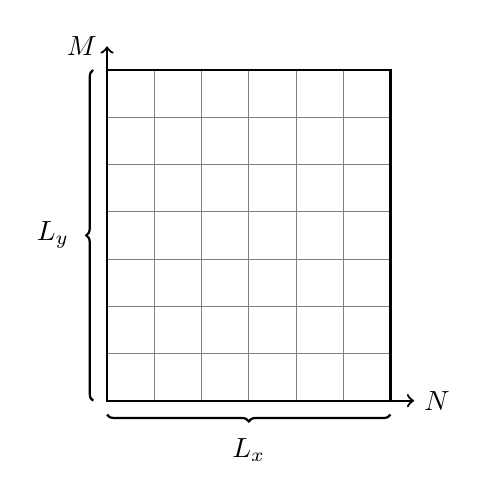
\begin{tikzpicture}[thick, scale=0.6]
\draw[step=1cm,gray,very thin] (-1,-1) grid (5,6);
\draw  (-1,-1) -- (5,-1) -- (5,6) -- (-1,6) -- (-1,-1);
\draw [<->] (-1,6.5) node [left]{$M$} -- (-1,-1) 
-- (5.5,-1) node [right] {$N$};
\draw [decoration={brace,mirror,raise=5pt},decorate]
(-1,-1) --  node[below=10pt]{$L_x$}(5,-1); 

\draw [decoration={brace,raise=5pt},decorate]
(-1,-1) --  node[left=10pt]{$L_y$}(-1,6); 

\end{tikzpicture}
\label{fig:stat1}
\end{SCfigure}
Wir betrachten nun 
die statistischen Eigenschaften der Zufallsvariablen $\xi(x,y)$. 
Die Wahrscheinlichkeitsdichte $\rho(x,y,z)$ für eine 
bestimmte Höhe $z$ ergibt sich numerisch
durch die Extrapolation der einzelnen Datenpunkte mit der Normierung:
\begin{equation*}
\int \rho(x,y,z) dx dy dz = 1
\end{equation*}
Nun lässt sich mithilfe von $\rho$ die 2-Punkt-Funktion
(2-point function) definieren:
\begin{equation}
w(\tau_x=x_1-x_2, \tau_y=y_1-y_2,z_1,z_2) = \rho(x_1,y_1,z_1)
\rho(x_2,y_2,z_2)
\end{equation}
Wobei wir die Abstände $\tau_x=x_1-x_2$ und $\tau_y=y_1-y_2,z_1,z_2$
definiert haben.
\subsubsection{Fouriertransformationenen und Autokorrelationsfunktion}
Sei nun ganz allgemein die Fouriertransformation eingeführt:
\begin{align}
f(x) &= \int_{-\infty}^{\infty} F(k)\exp(2\pi i kx)dk\\
F(k) &= \mathcal{F}_x\left [f(x)\right ](k) =
\int_{-\infty}^{\infty} f(k)\exp(-2\pi i kx)dx
\end{align}
Mit den (nur den wichtigsten) Eigenschaften:
\begin{align}
&\mathcal{F}\left [a f(x) + b g(x)\right ]
    = a F(k) + b G(k) 
    &\mbox{ (Linearität) }\\
&\mathcal{F}\left [f(x) * g(x)\right ](k)
    = \mathcal{F}\left [f(x)\right ]\mathcal{F}\left [g(x)\right ]
    \! &\mbox{ (Faltungseigenschaft) }\\
&\mathcal{F}_k\left [\left | F(k) \right |^2\right ](x)
   =  \int_{-\infty}^{\infty}\bar{f}(\tau)f(\tau + x) d\tau 
   &\mbox{ (Wiener-Khinchin Theorem) }
\end{align}
In der letzten Eigenschaft
bedeutet $\bar{f}$ die komplexe Konjugation von $f$.
Die Definitionen sind nun für die x-Richtung ausgeführt worden,
sie funktionieren jedoch analog im $2D$ Fall, also mit dem Tuple
$(x,y)$. 
Um das Leistungsspektrum berechnen zu können, führen wir 
nun die Autokorrelationsfunktion ein:
\begin{align}
    G(\tau_x,\tau_y) &=\int\int z_1 z_2 w(\tau_x,\tau_y,z_1,z_2) dz_1 dz_2 \mbox{ (Autokorrelationsfunktion) }\\
&= \int\int \xi(x_1,y_1)\xi(x_1+\tau_x,y_1+\tau_y)dx_1dy_1
\end{align}
Diese Funktion lässt sich nun auch diskret berechnen:
\begin{equation}
    G(m,n)=\frac{1}{(N-n)(M-m)}\sum_{l=1}^{N-n}\sum_{k=1}^{M-m}z_{k+m,l+n}z_{k,l}
\end{equation}
wobei $m=\tau_x/\Delta_x$ und $n=\tau_y/\Delta_y$. Die 2D-Autokorrelationsfunktion
(\textit{2D-Autocorrelationfunction}, kurz ACF) lässt sich auch im Vorfeld dazu verwenden,
statistische Daten nach ihrer Korrelation aufzutragen und somit Störungen herauszufiltern.
Sie wird häufig in der Spektroskopie (\textit{Correlationspectroscopy}) verwendet, um überlappende
Peaks in einer Dimension mithilfe einer 2D Darstellung zu trennen. In unserem Fall werden wir
die 2DAFC verwenden, um die durch die unperfekte Spitze enstehenden Einflüsse von den
Gittereigenschaften, die sich durch ihre Korrelationen bemerkbar machen, zu trennen.
Wie wir sehen, fügt sich nun die Vorarbeit nun zusammen und 
aus den unseren gemessenen diskreten Höhendaten lässt  
sich nun direkt die Autokorrelationsfunktion
berechnen. 
Um nun eine qualitative Aussage über die Verteilung der Moden
treffen zu können, berechnen wir das Leistungsspektrum (mithilfe
des Wiener-Khinchin Theorems):
\begin{align}
    W(K_x,K_y)=\frac{1}{4\pi}\int\int G(\tau_x,\tau_y)\exp(-i(K_x\tau_x+K_y\tau_y)) d\tau_xd\tau_y
\end{align}
Diese lässt sich wieder analog zur Autokorrelationsfunktion
für diskrete Werte berechnen. Wenn eine isotrope Struktur
vorläge, würde es sich nun anbieten, über die Fläche zu 
integrieren. Da dies bei unseren Proben nicht der Fall ist,
werden wir dies hier nicht weiter ausführen.\\

In der numerischen Analyse wird nun die ``Schnelle''
Fouriertransform (engl. \textit{Fast Fourier Transform, FFT})
berechnet. \\Da wir die Integraltransformationen
bei einem begrenzten und
nicht unendlichen Datensatz mit der
diskreten Fourier Transformation (DFT)
approximieren müssen, implizieren wir zyklische Randbedingungen:
\begin{align}
 &f(n) = \frac{1}{N}\sum_{n=0}^{N-1}{\exp(2\pi i \frac{kn}{N})f(k) }\\
 &F(k) = \sum_{n=0}^{N-1}{\exp(-2\pi i \frac{kn}{N})f(n) }
\end{align}
Da die realen Datensätze diese zyklischen
Randbedingungen nicht aufweisen, müssen
die Ränder des Datensatzes ``unterdrückt'' bzw. transformiert
werden. Generell wird dazu eine Fensterfunktion (\textit{Window
function}) verwendet, welche mit dem Signal gefaltet wird und
somit die bei der FFT auftretenden Randeffekte zu unterdrücken 
sucht (siehe Abbildung~\ref{fig:stm2}). 
Dabei sind verschiedene Windowfunctions
denkbar (siehe Abbildung~\ref{fig:windowing-fft},
welche über verschiedene
Güten verfügen und an die Eigenschaften
des Signals angepasst werden müssen.
\begin{figure}
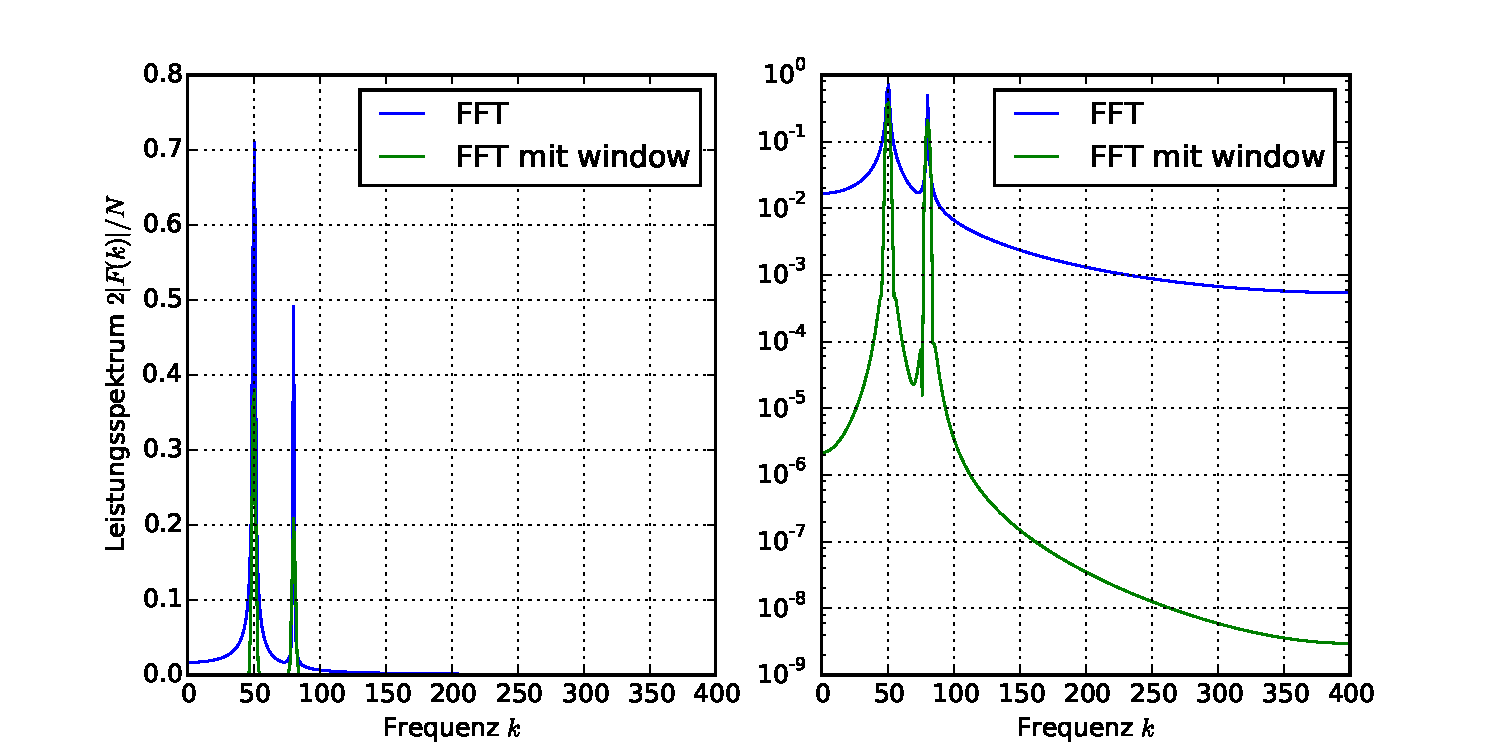
\includegraphics[width=17cm]{pics/stm2}
\caption{Hier berechnen wir numerisch die diskrete
    Fouriertransformation (FFT) des Signals  
$f(t)=\sin(2\pi \omega_1 t) + 0.5 \sin(2\pi \omega_2 t)$ mit den 
Frequenzen $\omega_1 = 50$ und $\omega_2 = 80$, jeweils mit
der Windowfunction \textit{blackman} und ohne. 
Die Berechnung erfolgte mit $N=600$ mithilfe der numerischen
Bibliothek \textit{numpy/scipy} in Python\cite{scipy_reference}.
Der Sourcecode dazu befindet sich im Anhang.
Wie aus den Diagrammen ersichtlich wird, bildet die windowfunktion
\textit{blackman} zusammen mit der FFT
die  beiden Frequenzen $\omega_1$ und $\omega_2$ viel besser ab
als die FFT alleine. Dies ist auch wichtig bei der Analyse der
Datenpunkte aus dem RTM, welche auch nur in diskret vorliegen.
}
 \label{fig:stm2}
\end{figure}

\begin{figure}
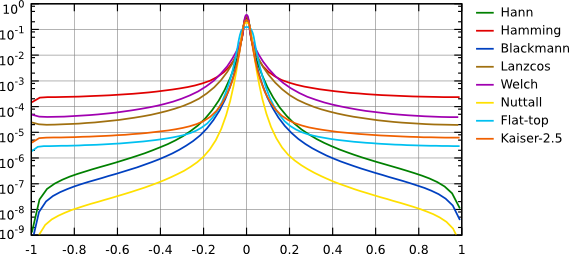
\includegraphics[width=12cm]{pics/windowing-fft}
\caption{Verschieden mögliche Windowfunktionen\cite{gwyddion}.
Die verschiedenen Funktionen unterscheidenen sich in ihrer
sogenannten \textit{Bandbreite}, das bedeutet, dass es keine
ideale Windowfunktion gibt, sondern dass jene an das Signal
angepasst werden muss. } 
\label{fig:windowing-fft}
\end{figure}

\subsubsection{Reziprokes Gitter und Fouriertransformationen}
Den Reziproken Raum (auch k-Raum genannt) erhält man durch die
Fouriertransformation des Ortsraumes. Somit erhalten wir durch
die Fouriertransformation des Gitters die erste Brillouin-Zone
des Reziproken Gitters. Deshalb bietet es sich an, mithilfe
des Leistungsspektrums der 2D-Fouriertransformation der 
Mikroskopiedaten die Gittereigenschaften der Probe zu analysieren
(Siehe Quelle \cite{kelty1991scanning}. In der Quelle wird zwar  
nicht explizit auf Methode eingegangen, sie wird allerdings
verwendet, um die Superstruktur von $KHgC_4$ in verschiedenen
Formen zu analysieren, siehe Abbildung~\ref{fig:powerspec}). 
\begin{figure}
    \begin{captionbeside}[]{Abbildungen aus \cite{kelty1991scanning}.
(a) Es handelt sich um eine 100x100 $\r{A}^2$ Rastertunnelmikroskopiebild
von $KHgC_4$ mit einem $8.9 \r{A}$ Gitterperiodenabstand.
(b) das 2DFT Power Spektrum, welches deutlich die Symmetrie des 
Supergitters und seine Orientierung zeigt.} 
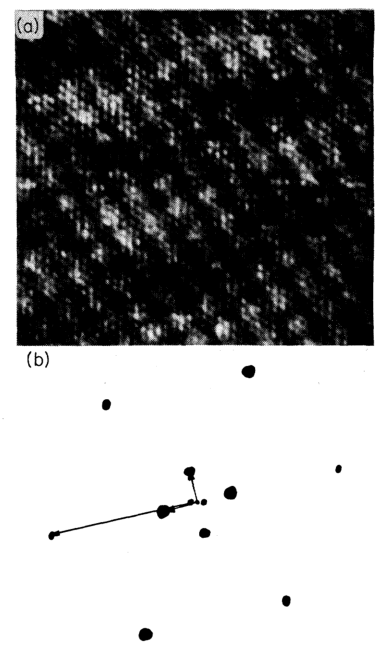
\includegraphics[width=6cm]{pics/powerspec}
\end{captionbeside}
\label{fig:powerspec}
\end{figure}


